%Especificacion
\documentclass[12pt]{scrartcl}

%Paquetes
\usepackage[left=2cm,right=2cm,top=3cm,bottom=3cm,letterpaper]{geometry}
\usepackage{lmodern}
\usepackage[T1]{fontenc}
\usepackage[utf8]{inputenc}
\usepackage{hyperref}
\usepackage{float}
\usepackage{caption}
\usepackage[spanish,activeacute]{babel}
\usepackage{mathtools}
\usepackage{amssymb}
\usepackage{enumerate}
%\usepackage{tabularx}
%\usepackage{wasysym}
\usepackage{graphicx}
\usepackage{pmboxdraw}
\graphicspath { {pics/} }
%\usepackage{pifont}
%Preambulo
\title{Sistemas Operativos\\ Guía visual: Instalación de Minix}
\subtitle{Profesor: Salvador López Mendoza }
\author{Andrea González Vargas \and Carlos Gerardo Acosta Hernández}
\date{Facultad de Ciencias UNAM \\ 2019-2}
\setlength\parindent{0pt}

\begin{document}
\maketitle


\tableofcontents
\newpage
\section{Prólogo}\label{prol}
Antes de comenzar la instalación, descargar la imagen ISO de \texttt{Minix 3} en la página oficial\footnote{\url{https://wiki.minix3.org/doku.php?id=www:download:start}}:
\begin{figure}[H]
  \centering
  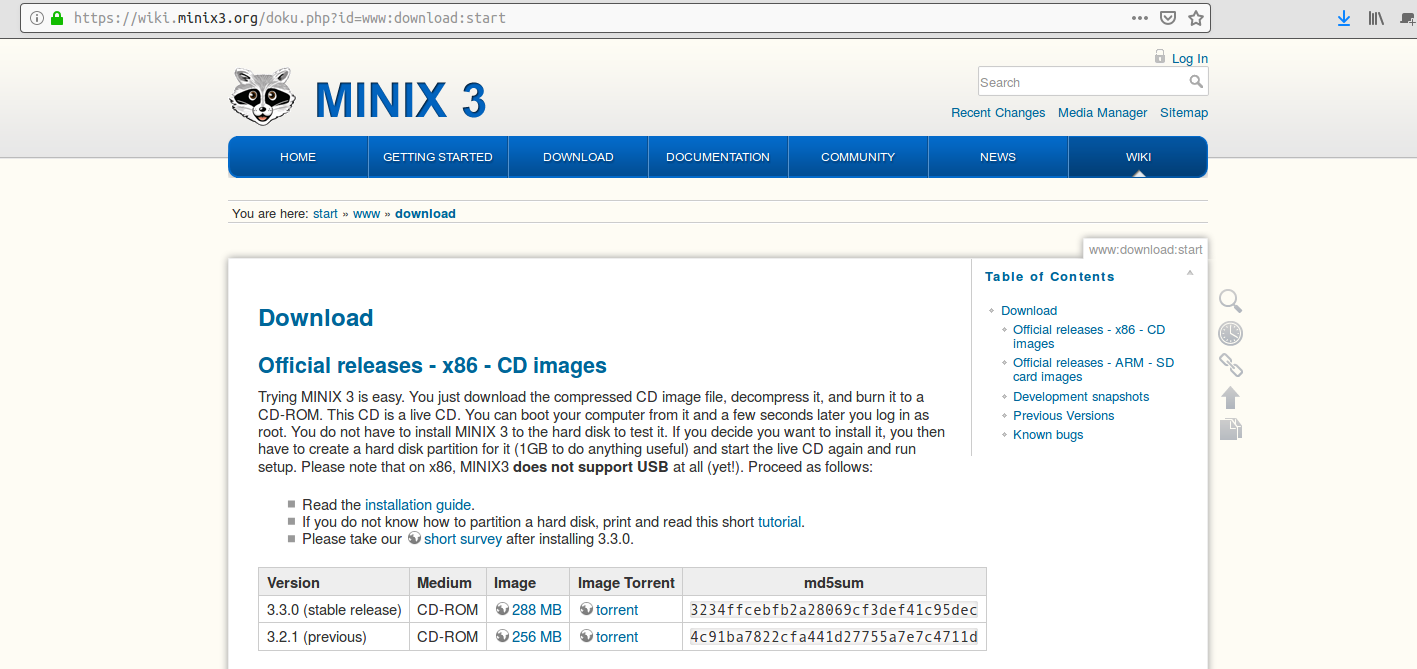
\includegraphics[width=\textwidth]{vm/min00.png}
  \caption{Página oficial de descarga de \texttt{Minix 3}}
\end{figure}

Proseguir a seguir las instrucciones del virtualizador que vaya a utilizarse (VMWare o VirtualBox):
\newpage

\section{VMWare}

\subsection{Preparación de la máquina virtual}

Crear una nueva máquina virtual accediendo a \textit{File $\rightarrow$ New\ Virtual\ Machine}.\\

Escoger la configuración de tipo \textit{Typical}.
\begin{figure}[H]
  \centering
  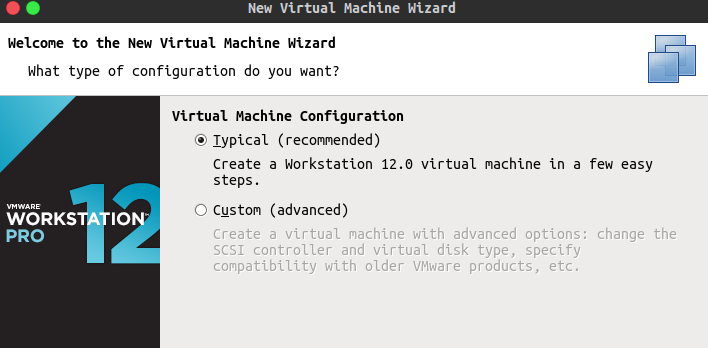
\includegraphics[width=0.6\textwidth]{vm/min01.png}
  \caption{Creación de nueva máquina virtual}
\end{figure}

Indicar que se instalará el sistema operativo después de la creación de la máquina virtual.
\begin{figure}[H]
  \centering
  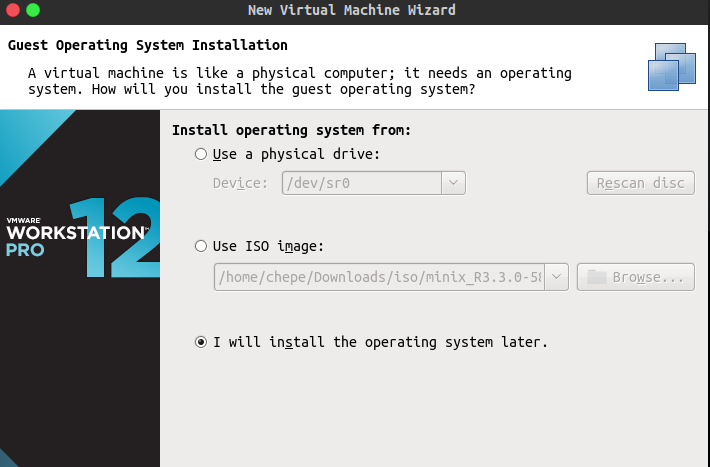
\includegraphics[width=0.6\textwidth]{vm/min02.png}
  \caption{Opciones de sistema operativo}
\end{figure}

Seleccionar \textit{Other} para el tipo de sistema operativo a instalar.
\begin{figure}[H]
  \centering
  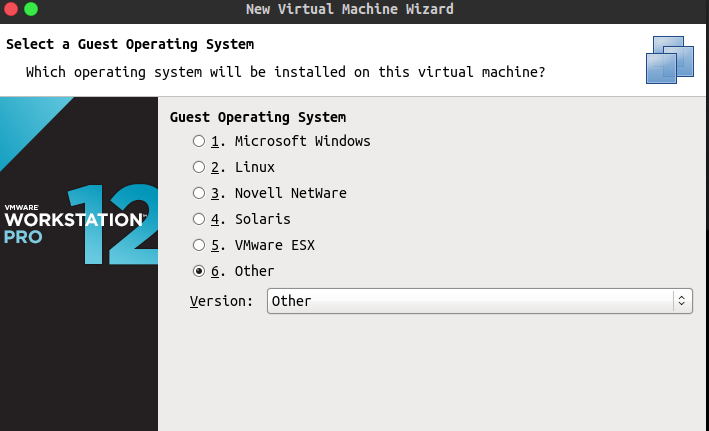
\includegraphics[width=0.6\textwidth]{vm/min03.png}
  \caption{Tipo de sistema operativo a instalar}
\end{figure}

Nombrar máquina e indicar la ruta de creación.
\begin{figure}[H]
  \centering
  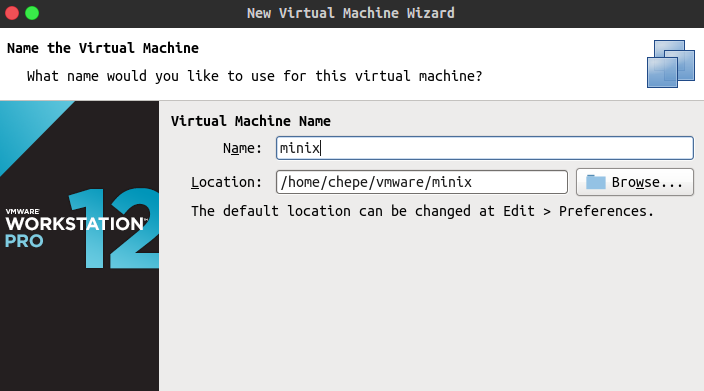
\includegraphics[width=0.6\textwidth]{vm/min04.png}
  \caption{Ruta de creación de máquina}
\end{figure}

Indicar el tamaño del disco duro (se recomienda crear disco de 2GB).
\begin{figure}[H]
  \centering
  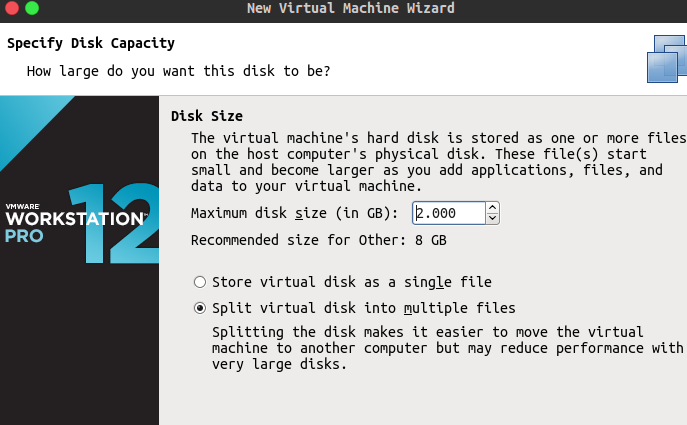
\includegraphics[width=0.6\textwidth]{vm/min05.png}
  \caption{Tamaño de disco duro}
\end{figure}

Seleccionar la opción \textit{Customize Hardware...}.
\begin{figure}[H]
  \centering
  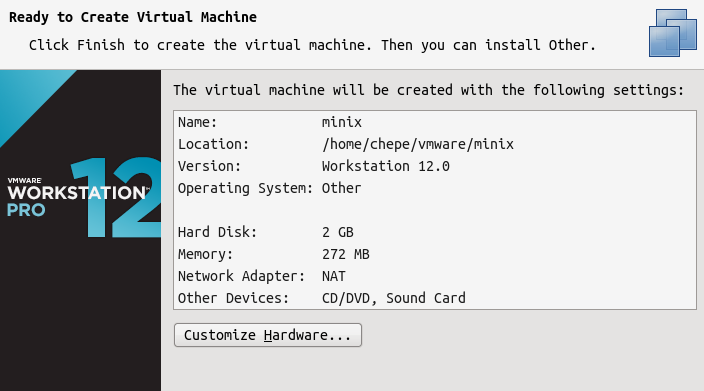
\includegraphics[width=0.6\textwidth]{vm/min10.png}
  \caption{Vista de configuraciones}
\end{figure}

Aumentar el tamaño de la memoria RAM a 512 MB.
\begin{figure}[H]
  \centering
  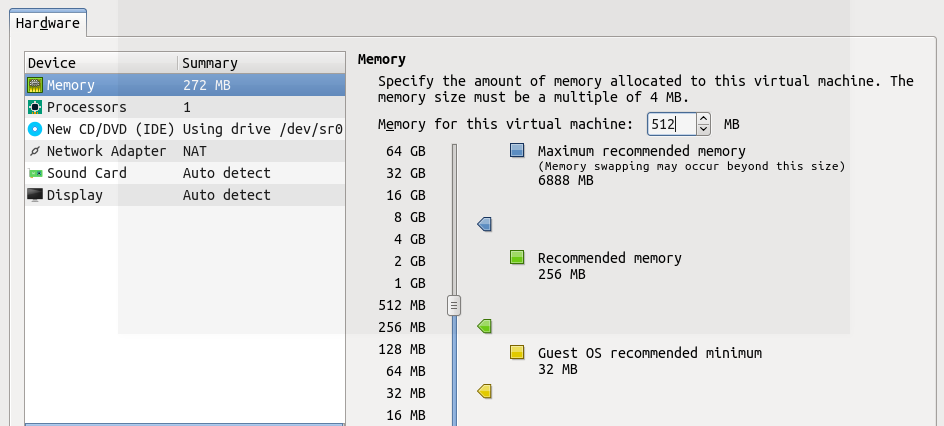
\includegraphics[width=0.6\textwidth]{vm/min11.png}
  \caption{Configuraciones de \textit{Hardware}}
\end{figure}

\subsection{Inicio del sistema (Pre-Instalación)}
Terminar creación de máquina virtual, seleccionar opción \textit{Edit virtual machine settings}.
\begin{figure}[H]
  \centering
  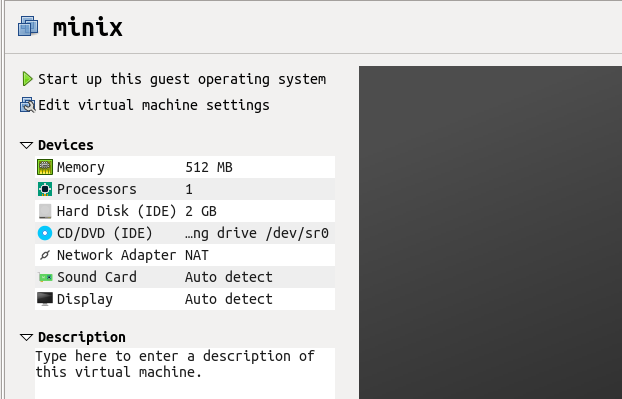
\includegraphics[width=0.6\textwidth]{vm/min13.png}
  \caption{Vista de máquina virtual}
\end{figure}

Dentro de las opciones del dispositivo CD/DVD, seleccionar \textit{Use ISO image} y elegir la imagen ISO previamente descargada de \texttt{Minix 3}.
\begin{figure}[H]
  \centering
  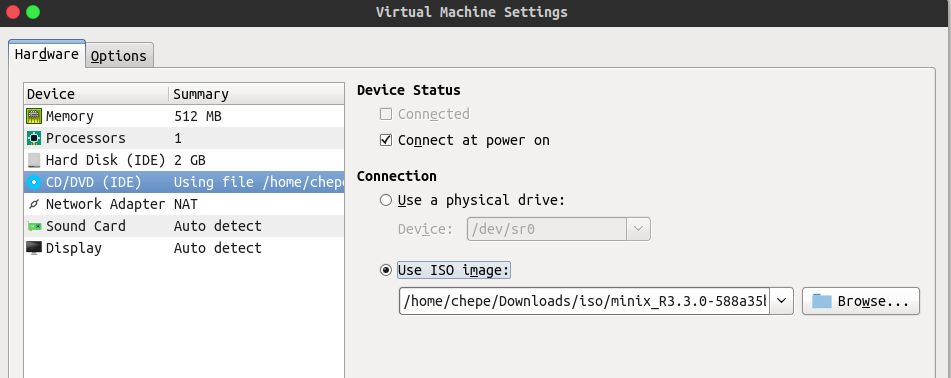
\includegraphics[width=0.6\textwidth]{vm/min14.png}
  \caption{Configuraciones de máquina virtual}
\end{figure}

Prender máquina y comenzar con la instalación del sistema operativo \ref{instalacion}.\\

\subsection{Inicio del sistema (Post-Instalación)}\label{vm:post}
Una vez instalado el sistema operativo, apagar máquina, ingresar a las configuraciones del sistema operativo, modificar opciones del dispositivo CD/DVD y seleccionar la opción \textit{Use a physical drive}.

\begin{figure}[H]
  \centering
  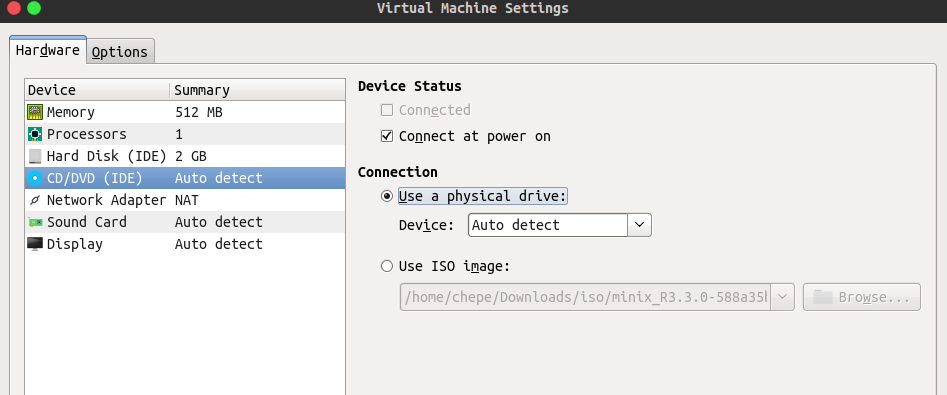
\includegraphics[width=0.6\textwidth]{vm/min32.png}
  \caption{Configuraciones de máquina virtual}
\end{figure}

Al prender la máquina se podra ingresar al sistema operativo ya instalado iniciando sesión como el usuario \texttt{root}.
\begin{figure}[H]
  \centering
  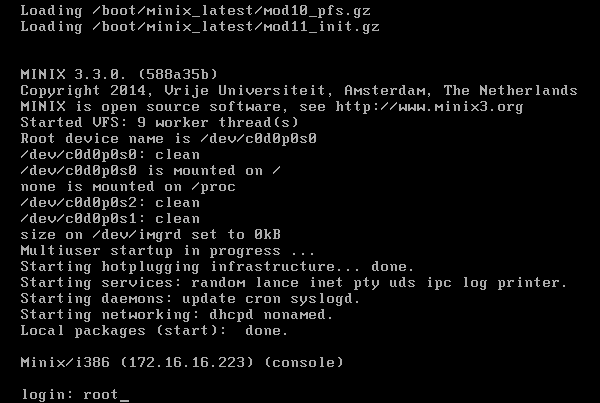
\includegraphics[width=0.6\textwidth]{vm/min33.png}
  \caption{Inicio de sesión}
\end{figure}

\newpage
\section{VirtualBox}

\subsection{Preparación de la máquina virtual}

Comenzar la configuración de una nueva máquina virtual haciendo clic en el botón \textit{Add}.\\
Rellenar la información que solicita el asistente.
\begin{figure}[H]
  \centering
  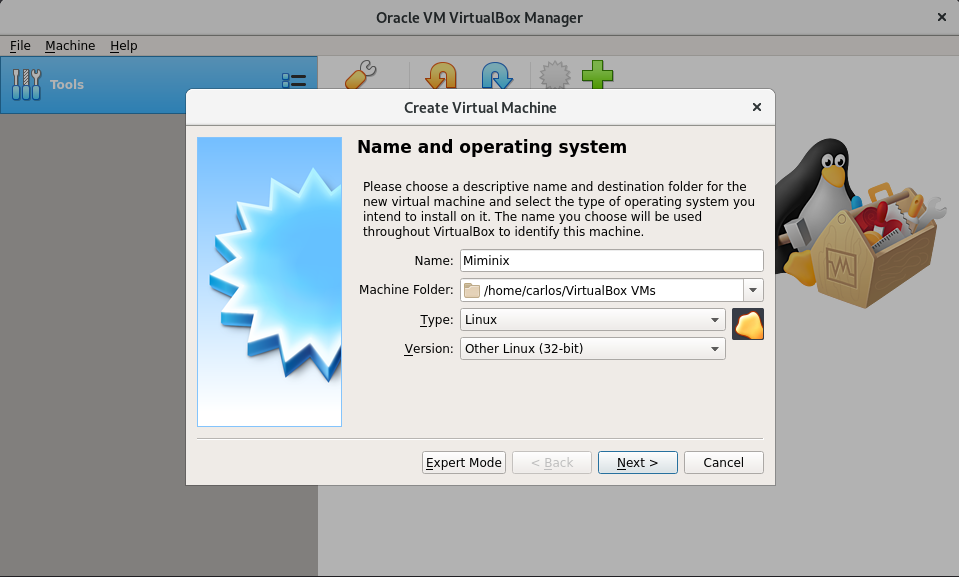
\includegraphics[width=0.66\textwidth]{vb/1.png}
  \caption{Inicio del asistente de creación de una nueva máquina virtual}
\end{figure}

A continuación asignar una cantidad de memoria (\textit{RAM}) para la nueva máquina virtual.
Procurar que sea mayor a 128 MB, pues \textit{Minix} requiere al menos esta cantidad para su recompilación en esta versión.

\begin{figure}[H]
  \centering
  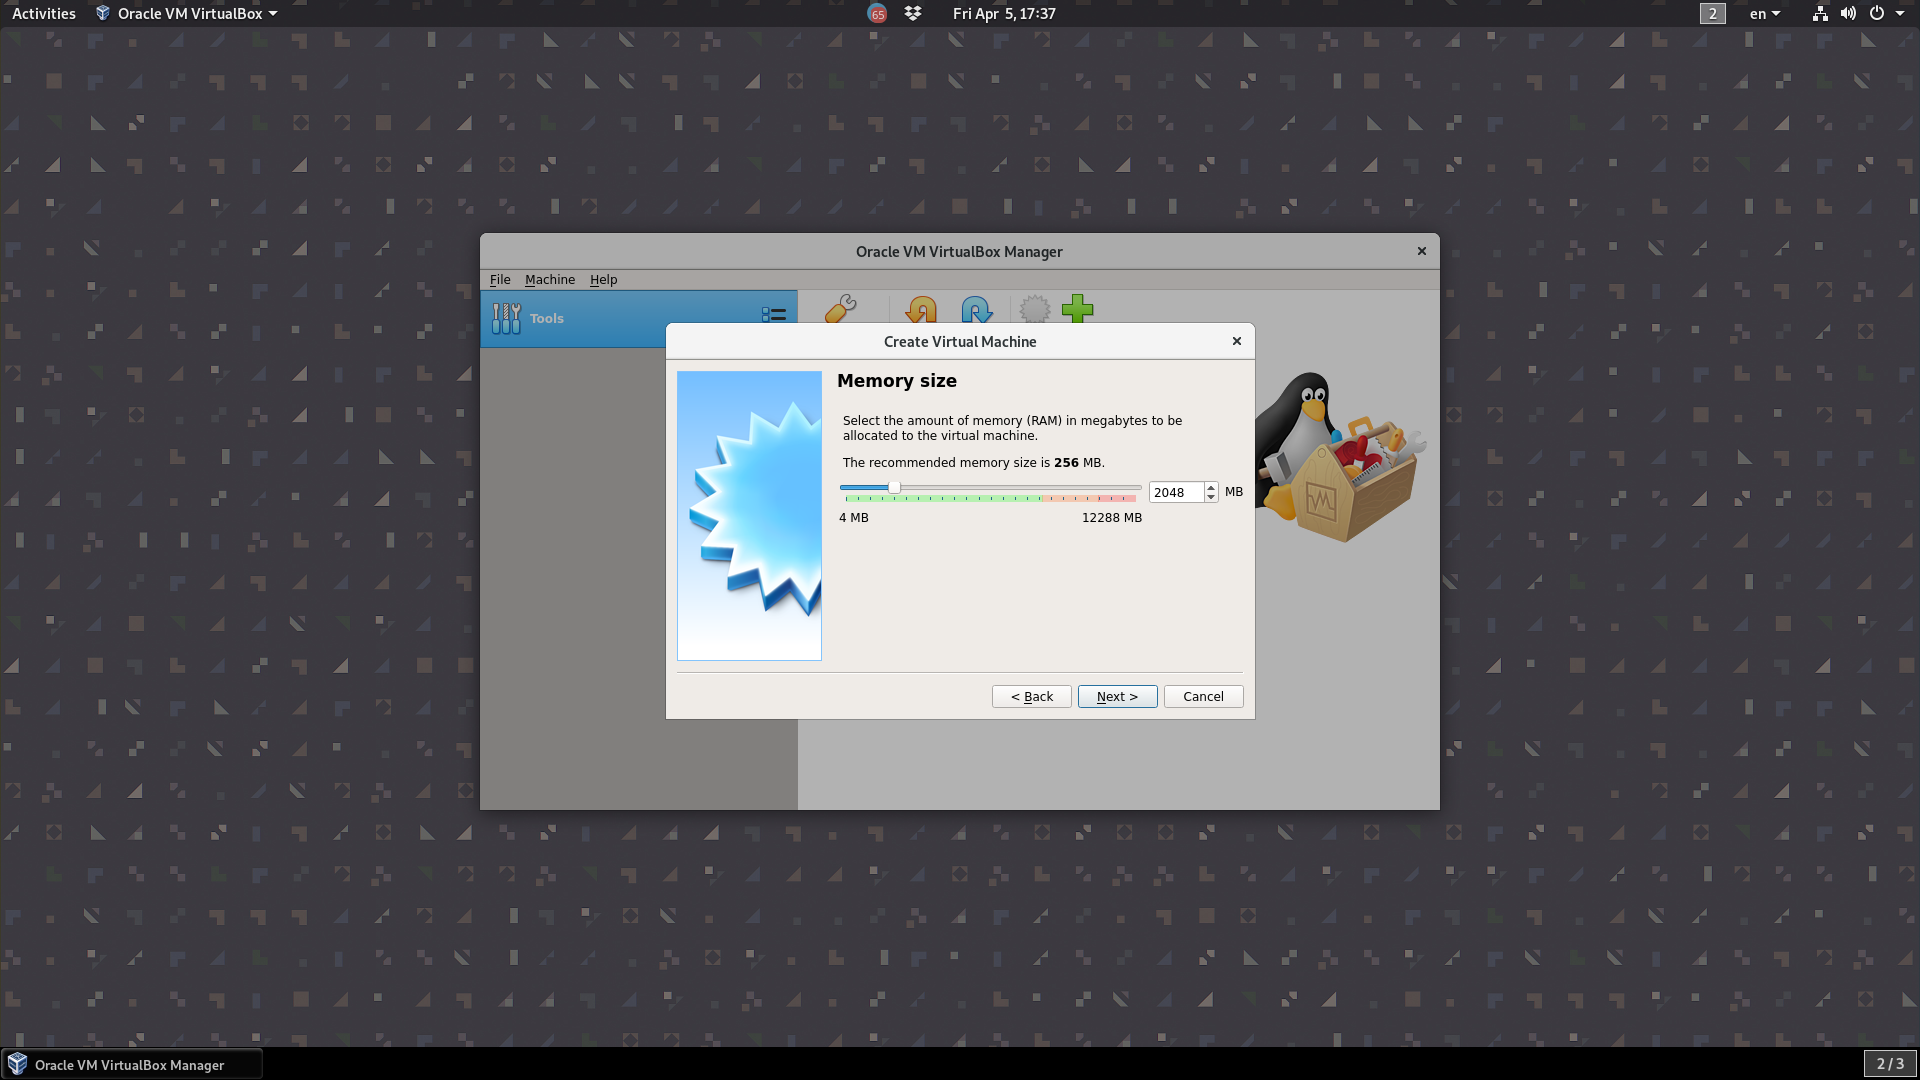
\includegraphics[width=0.66\textwidth]{vb/2.png}
  \caption{Tamaño de memoria exagerado para \textit{Minix}}
\end{figure}

Crear un disco duro virtual\footnote{También es posible reutilizar algún otro, preferentemente ya particionado.} donde será instalado \textit{Minix}.
\begin{figure}[H]
  \centering
  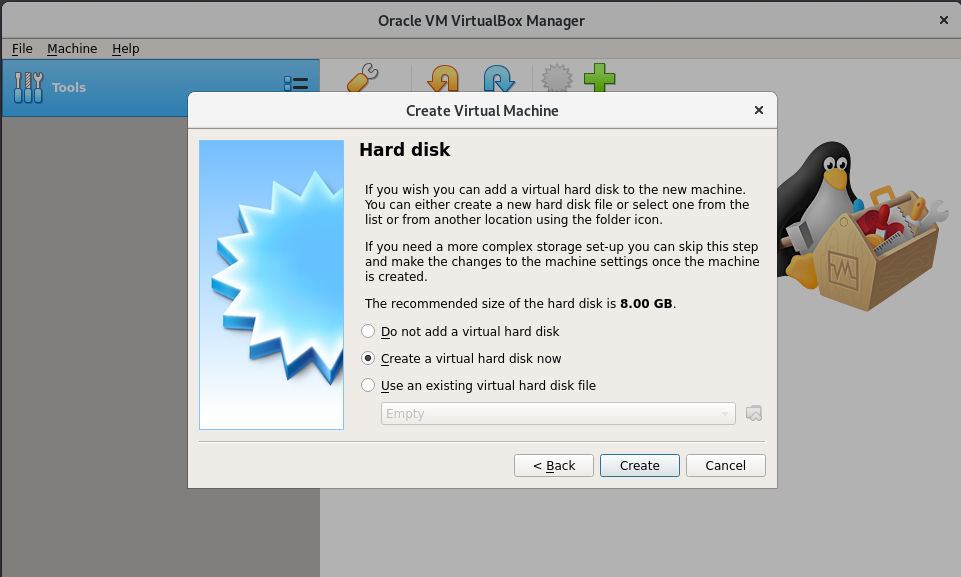
\includegraphics[width=0.68\textwidth]{vb/3.png}
  \caption{Creación de una unidad de disco duro virtual}
\end{figure}

Escoger el formato \textbf{VMDK}, pues a pesar de ser desarrollado inicialmente como formato nativo de \textit{VMWare}, es soportado por múltiples
programas de virtualización; tales como \textit{VirtualBox}, \textit{Sun xVM}, \textit{QEMU}, \textit{SUSE Studio}, \textit{.NET DiscUtils}, entre otros.
\begin{figure}[H]
  \centering
  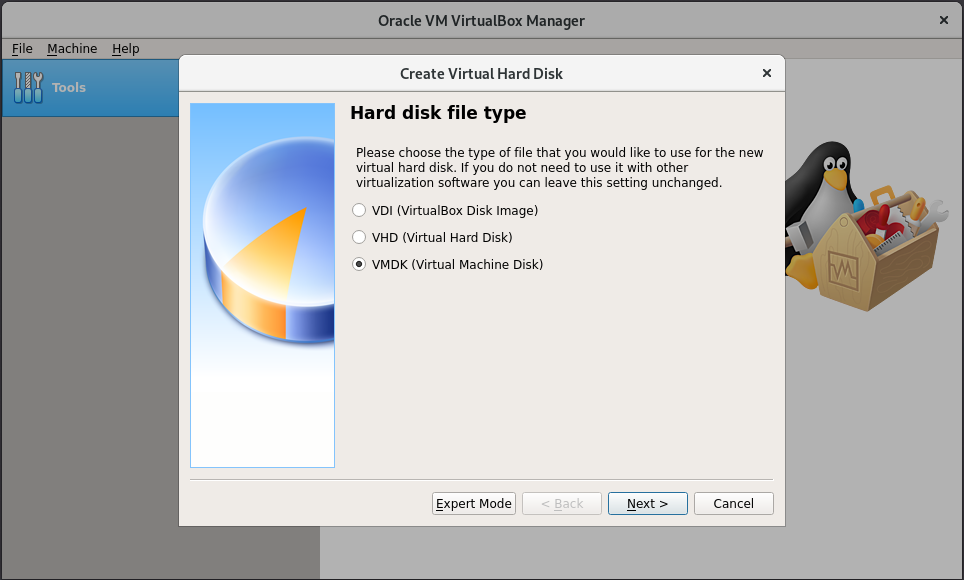
\includegraphics[width=0.68\textwidth]{vb/4.png}
  \caption{Formato de archivo del contenedor de disco duro virtual }
\end{figure}
\newpage
Decidir qué tipo de almacenamiento en el disco duro físico (máquina anfitriona) se utilizará. Considerar que de tener no conocer el alcance del tamaño de la máquina virtual en el sistema anfitrión elegir la opción \textit{dynamically allocated/reservado dinámicamente} puede ser la mejor opción.  
\begin{figure}[H]
  \centering
  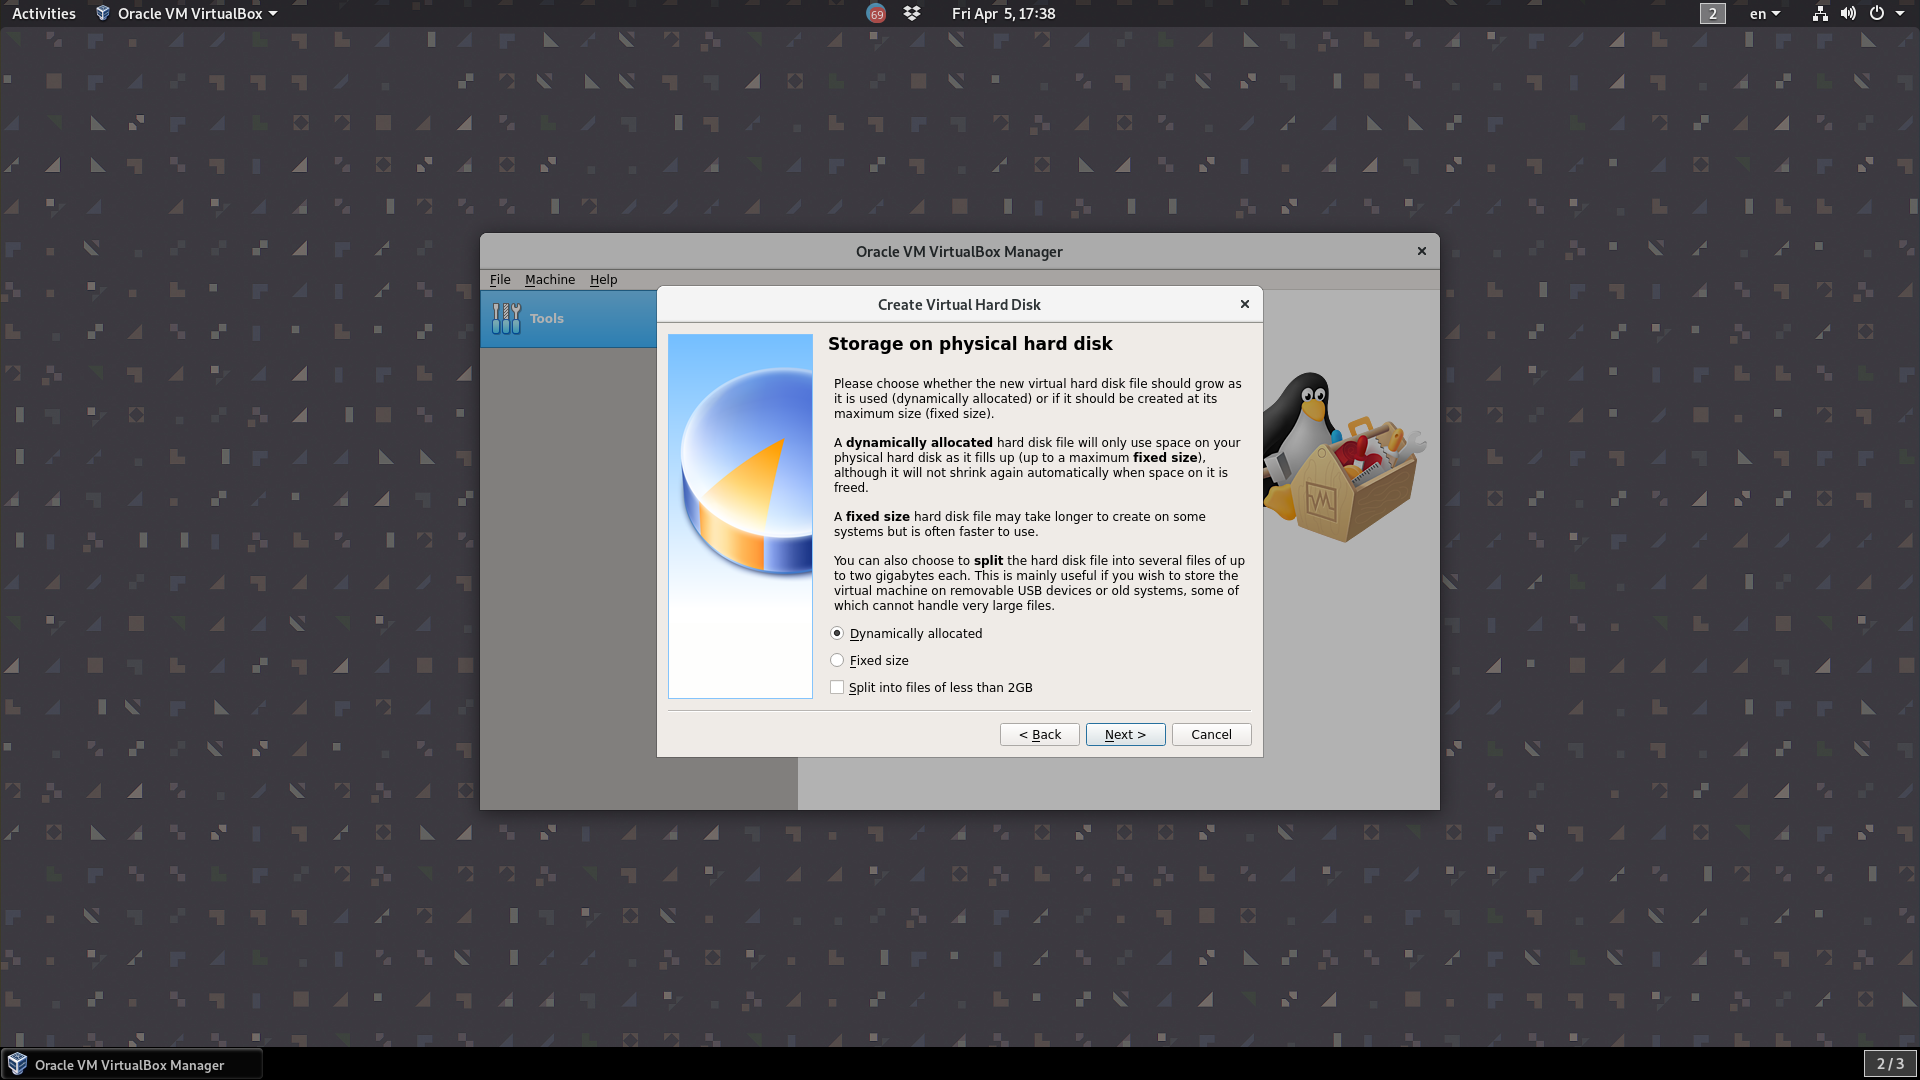
\includegraphics[width=0.66\textwidth]{vb/5.png}
  \caption{Manejo del espacio a ocupar por la unidad de disco duro virtual en el sistema anfitrión}
\end{figure}

Es posible definir un límite al almacenamiento al tamaño máximo de la máquina huésped en el disco duro de nuestro sistema anfitrión, aunque crezca dinámicamente.
Es importante asignar más de 360 MB para que el sistema pueda funcionar correctamente, sin embargo, quizá sea preferible proporcionarle cuando menos 1.2 GB, considerando la posibilidad agregar una interfaz gráfica, el código fuente de todo el sistema y las posteriores recompilaciones que se realicen.

\begin{figure}[H]
  \centering
  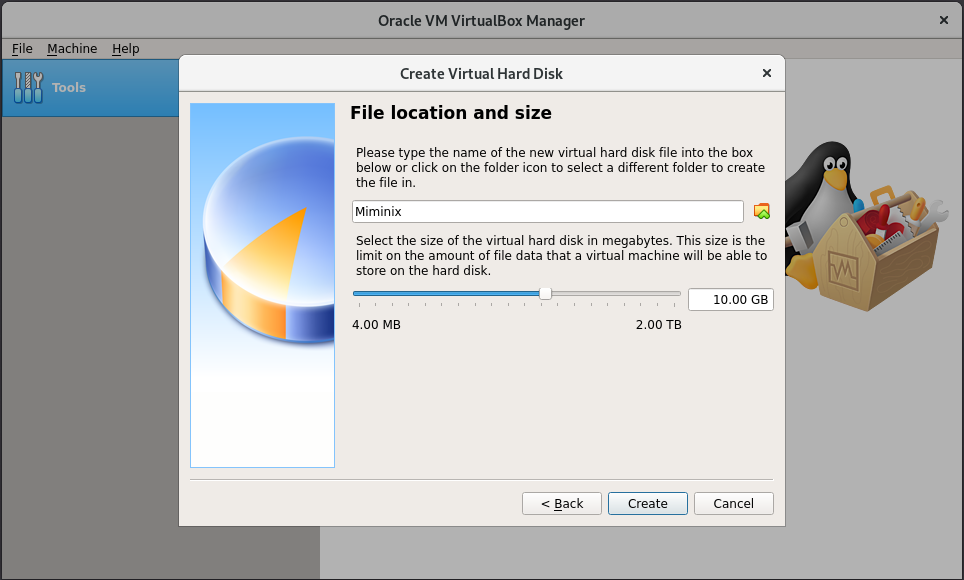
\includegraphics[width=0.66\textwidth]{vb/6.png}
  \caption{Límite exagerado para el sistema operativo \textit{Minix}}
\end{figure}

Al finalizar, se pueden verificar los detalles de la máquina virtual recién creada desde el administrador de \textit{VirtualBox}.

\begin{figure}[H]
  \centering
  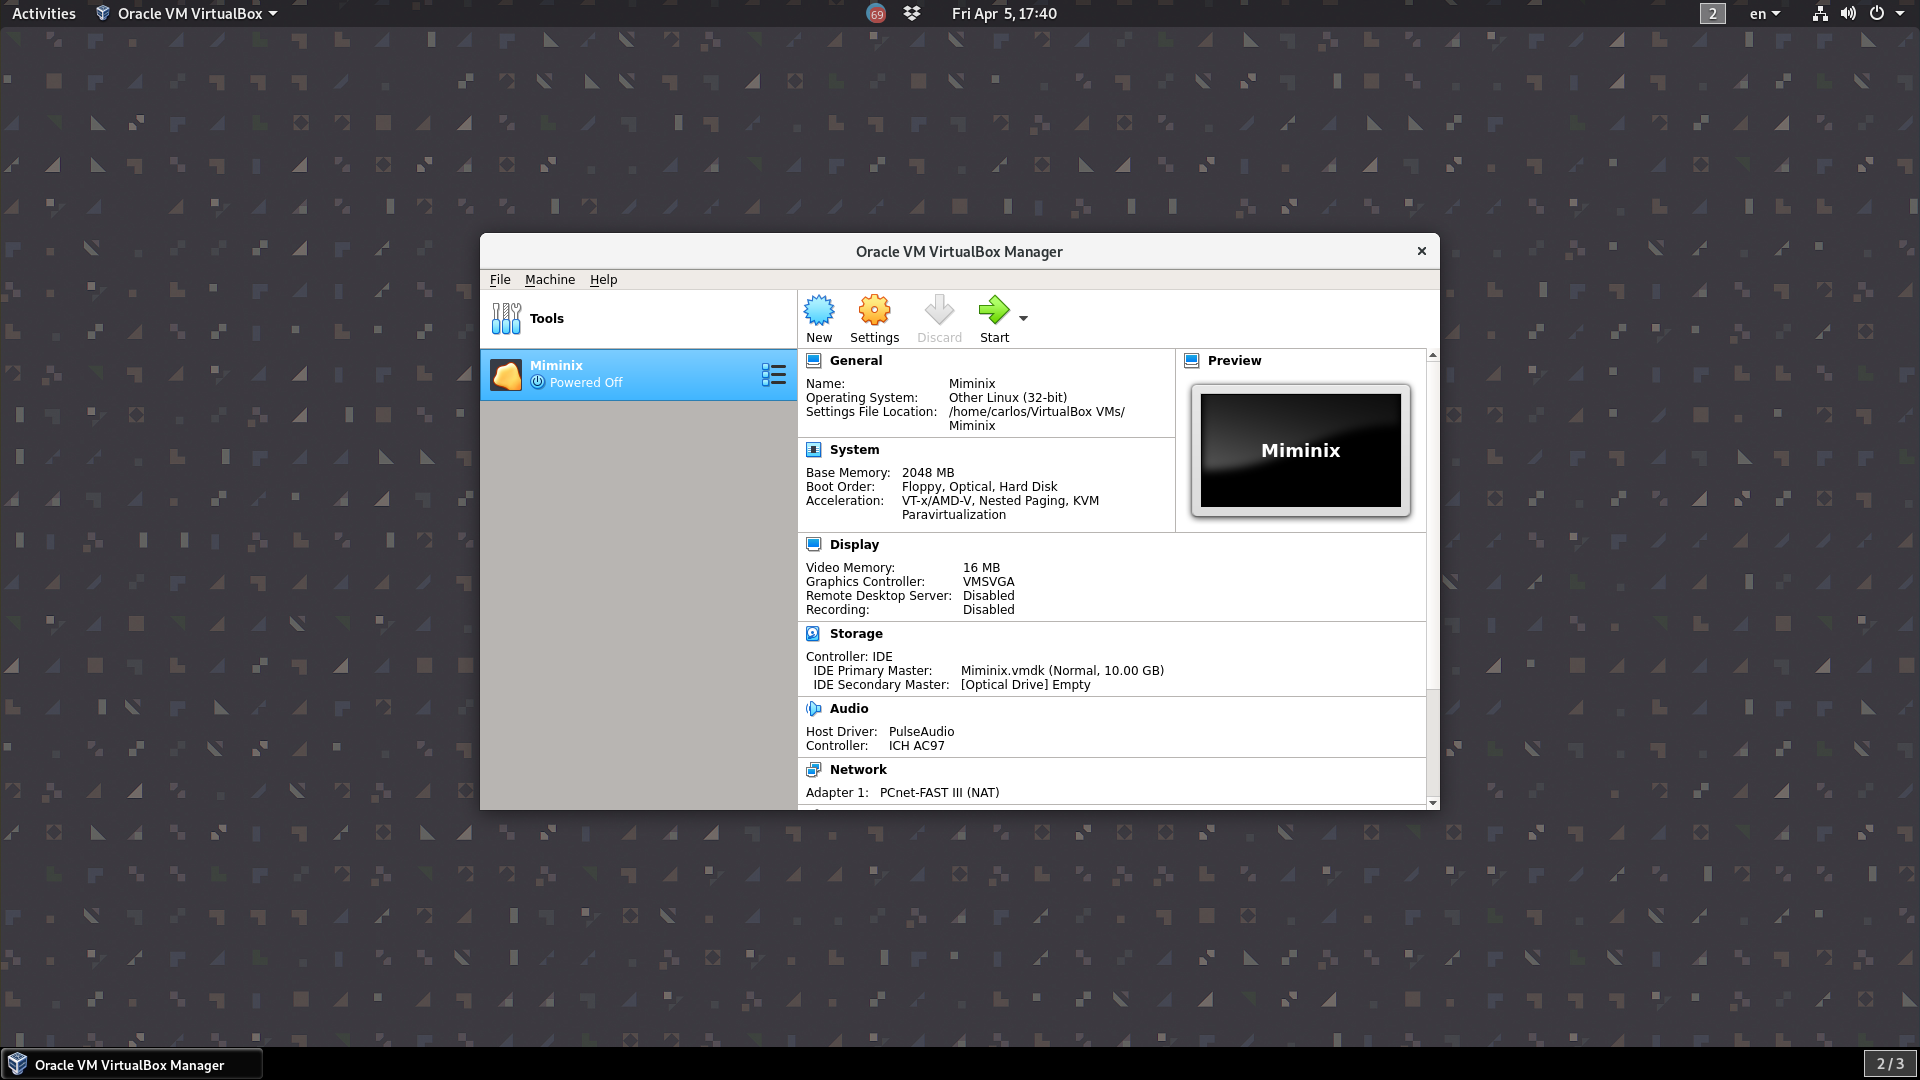
\includegraphics[width=0.8\textwidth]{vb/7.png}
  \caption{Detalles de la máquina virtual}
\end{figure}

\subsection{Inicio del sistema (Pre-Instalación)}
Para agregar el medio de instalación de \textit{Minix} como disco óptico, acceder a \textit{Settings/Configuración} $\rightarrow$  \textit{Storage/Almacenamiento}.

\begin{figure}[H]
  \centering
  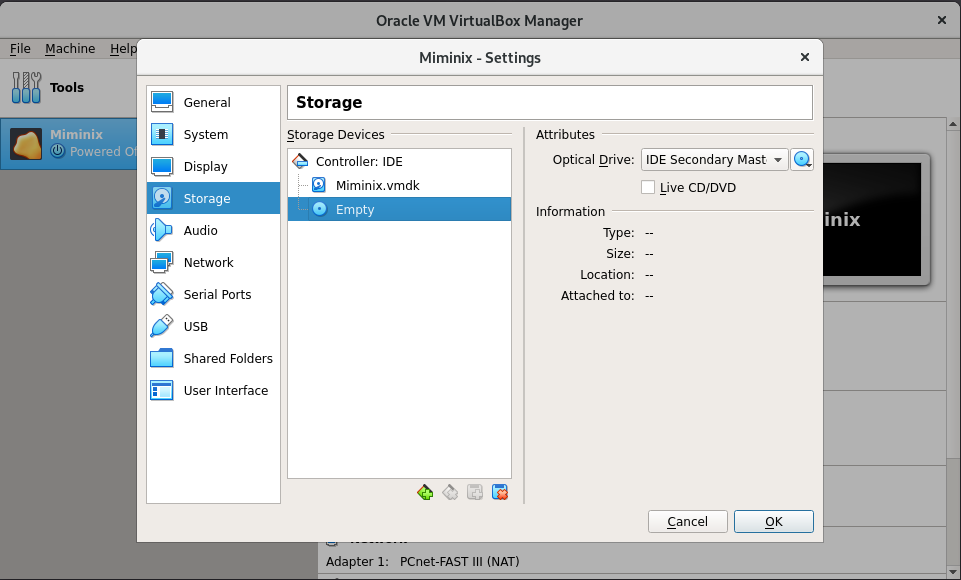
\includegraphics[width=0.66\textwidth]{vb/8.png}
  \caption{Selección de la entrada en la unidad óptica vacía}
\end{figure}

Dar clic en el botón del disco azul en el extremo derecho para seleccionar un archivo de disco óptico virtual para su carga en la unidad óptica virtual. Se deberá escoger el archivo imagen de instalación de \textit{Minix} en la ruta de su descarga (ver \ref{prol}).
\begin{figure}[H]
  \centering
  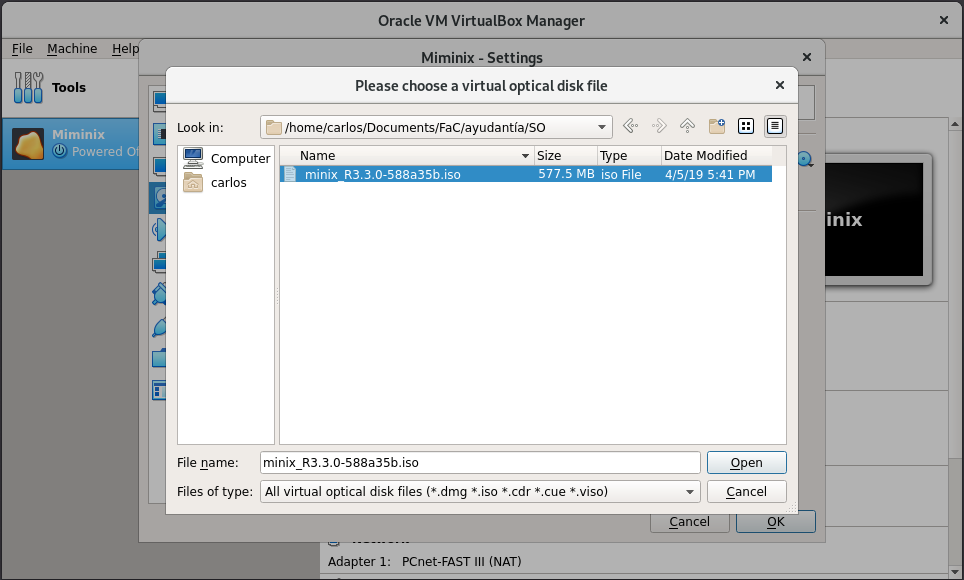
\includegraphics[width=0.66\textwidth]{vb/9.png}
  \caption{Selección del archivo imagen de disco con extensión \textit{.iso}}
\end{figure}

Al finalizar, deberá aparecer en los detalles, bajo la sección de almacenaiento, la unidad óptica ocupada por el archivo de imagen de disco de \textit{Minix} que se eligió.

\begin{figure}[H]
  \centering
  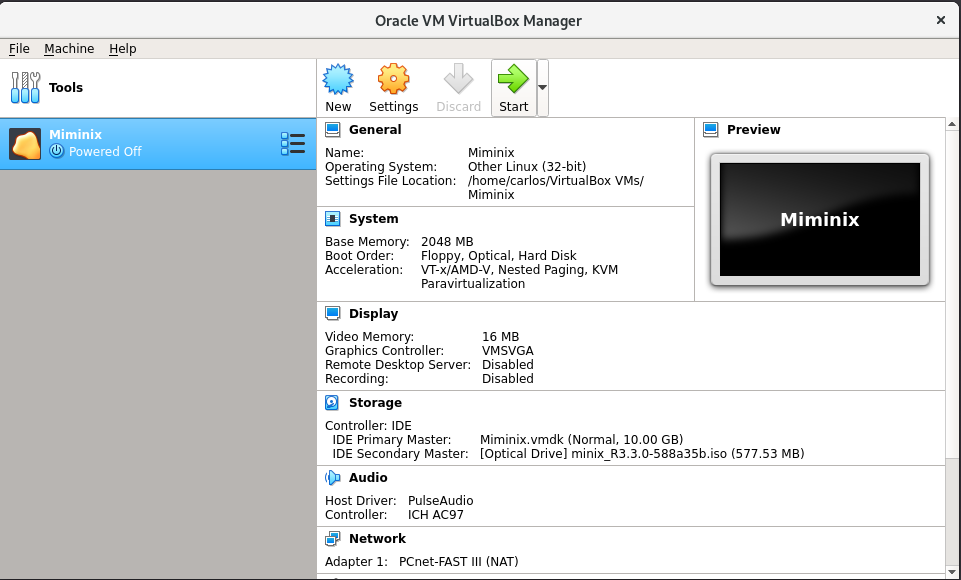
\includegraphics[width=0.8\textwidth]{vb/10.png}
  \caption{}
\end{figure}

Con esto se podrá continuar a la instalación (ver \ref{instalacion}) del sistema operativo una vez que se encienda la máquina virtual con \textit{Start/Iniciar}.

\subsection{Inicio del sistema (Post-Instalación)}\label{vb:post}

Una vez instalado el sistema operativo, será necesario retirar de la unidad óptica virtual el archivo de imagen de disco de \textit{Minix}. De esta forma, la máquina virtual iniciará el arranque del disco duro virtual donde se aloja ya la nueva instalación del sistema operativo.
\begin{figure}[H]
  \centering
  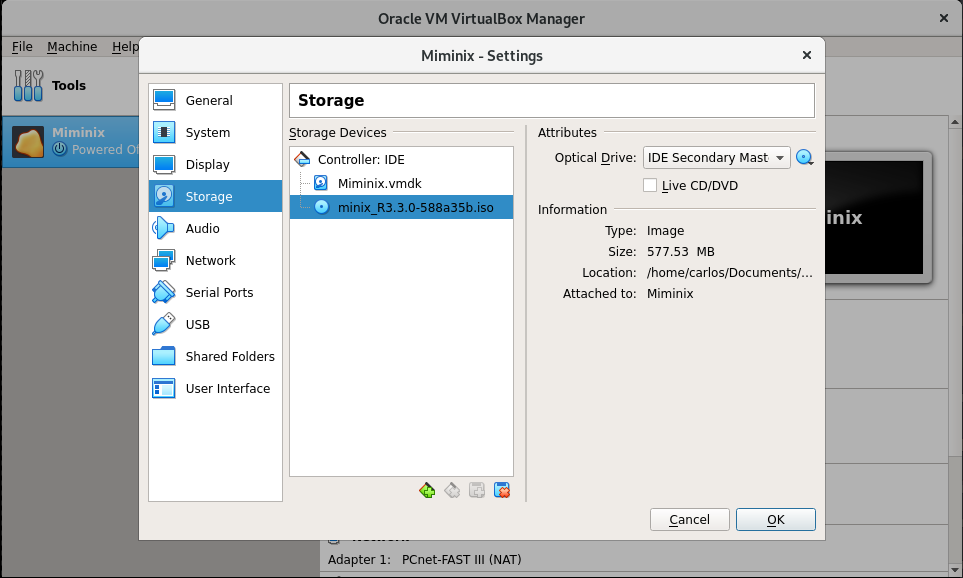
\includegraphics[width=0.8\textwidth]{vb/25.png}
  \caption{Selección de la unidad optica virtual del sistema huésped.}
\end{figure}

Seleccionar el botón del disco azul en el extremo derecho y dar clic en la opción de \textit{Remove Disk from virtual drive/Eliminar disco de la unidad virtual}.
Comprobar que en la sección de dispositivos de almacenamiento la unidad óptica se marque vacía. 
\begin{figure}[H]
  \centering
  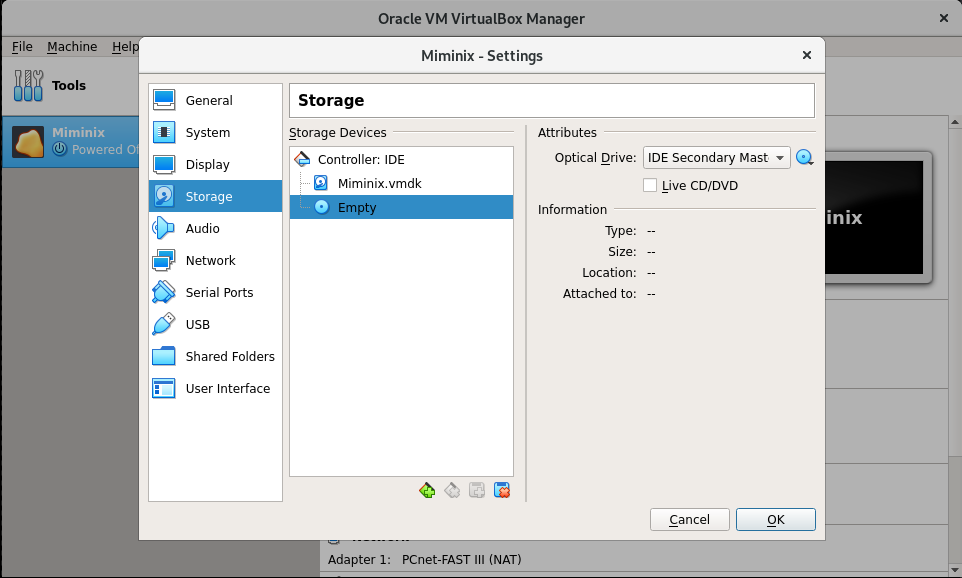
\includegraphics[width=0.8\textwidth]{vb/26.png}
  \caption{}
\end{figure}

Aceptar los cambios, verificar nuevamente que en los detalles generales de la máquina virtual aparezca la unidad óptica vacía y prenderla para comprobar la persistencia de la instalación.

\begin{figure}[H]
  \centering
  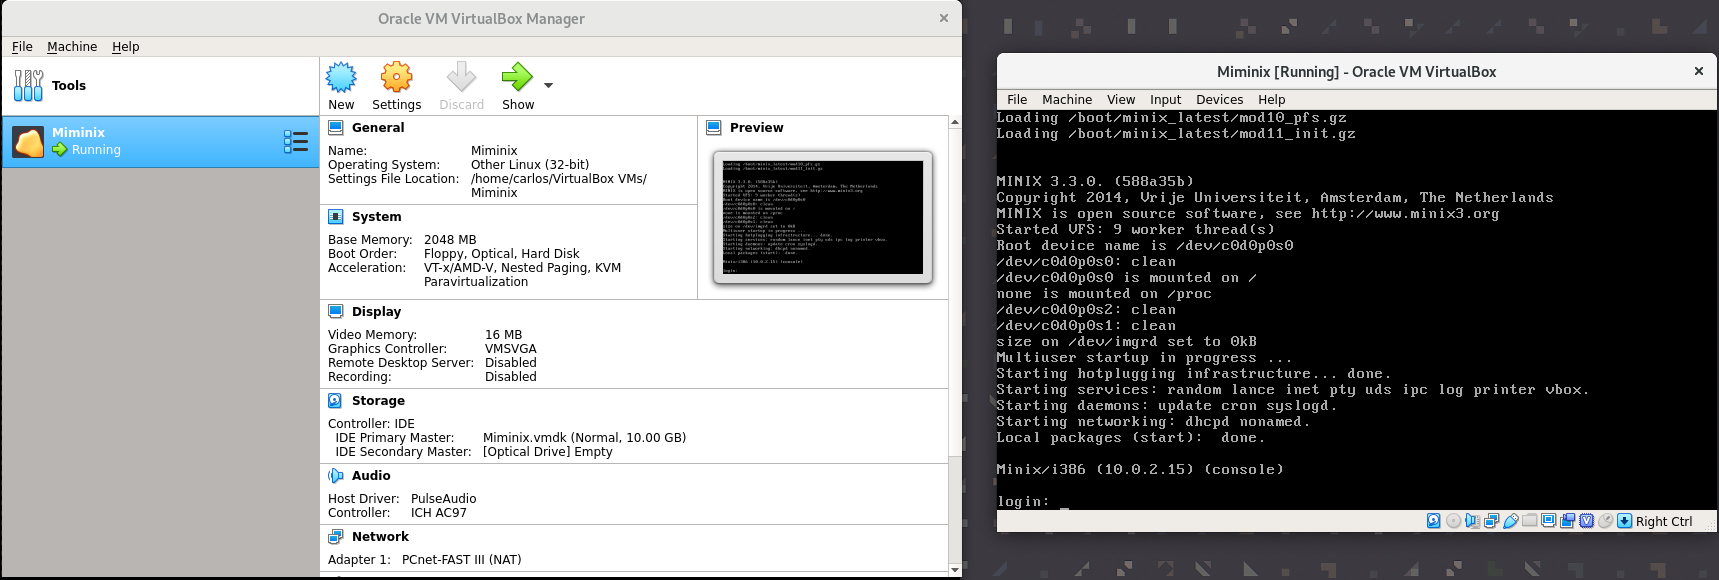
\includegraphics[width=1\textwidth]{vb/28.png}
  \caption{}
\end{figure}

\newpage
\section{Instalación de sistema operativo}\label{instalacion}

Seleccionar la primera opción que se muestra al prender la máquina para iniciar la instalación del sistema.
\begin{figure}[H]
  \centering
  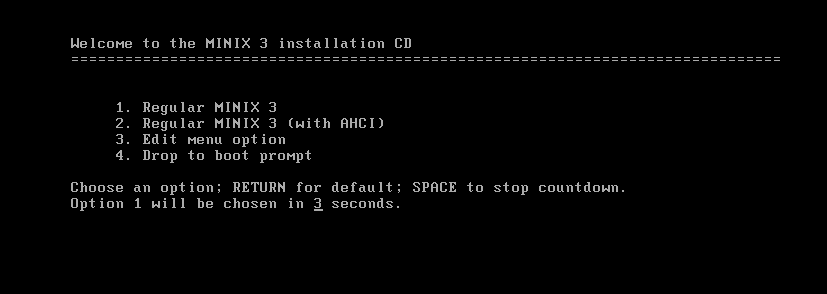
\includegraphics[width=0.7\textwidth]{vm/min15.png}
  \caption{Opciones de inicio}
\end{figure}

Iniciar sesión como el usuario \texttt{root}.
\begin{figure}[H]
  \centering
  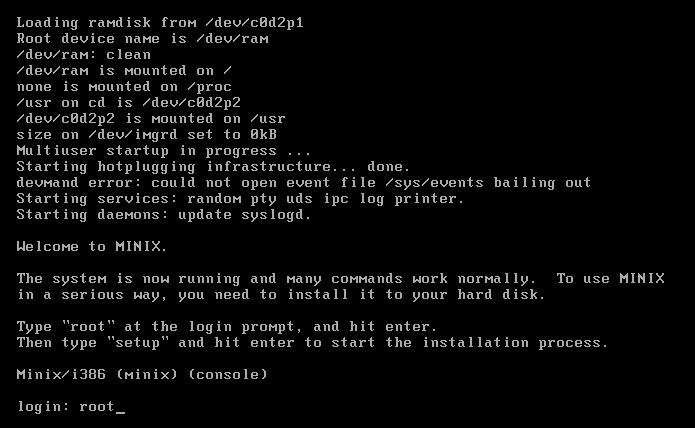
\includegraphics[width=0.7\textwidth]{vm/min16.png}
  \caption{Inicio de sesión}
\end{figure}

\subsection{Configuración de instalación}

Proceder con la instalación ingresando el comando \texttt{setup}.
\begin{figure}[H]
  \centering
  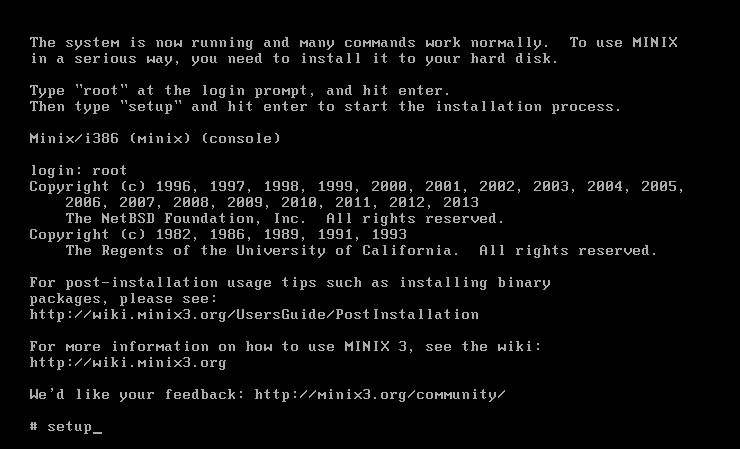
\includegraphics[width=0.7\textwidth]{vm/min18.png}
  \caption{Inicio de instalación}
\end{figure}

\subsubsection{Distribución de teclado}
Escoger el tipo de teclado a utilizar, en este caso se seleccionó la opción \texttt{latin-america}.
\begin{figure}[H]
  \centering
  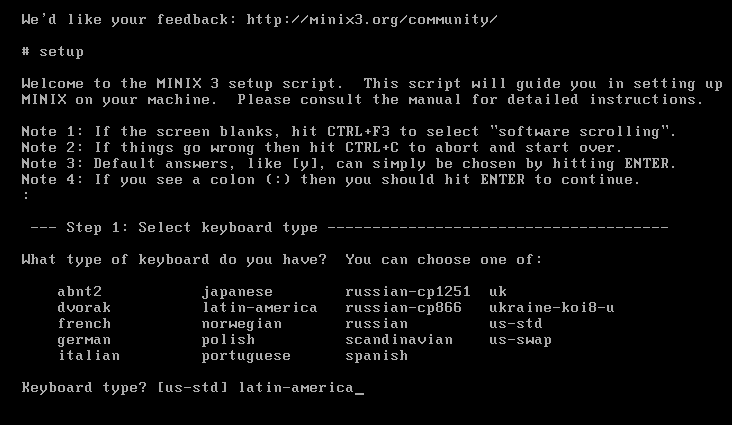
\includegraphics[width=0.7\textwidth]{vm/min19.png}
  \caption{Selección de tipo de teclado}
\end{figure}

\subsubsection{Disco objetivo de instalación}
Crear la partición para la instalación de sistema operativo, en este caso se escogió el modo automático al presionar la tecla \texttt{[ENTER]}.
\begin{figure}[H]
  \centering
  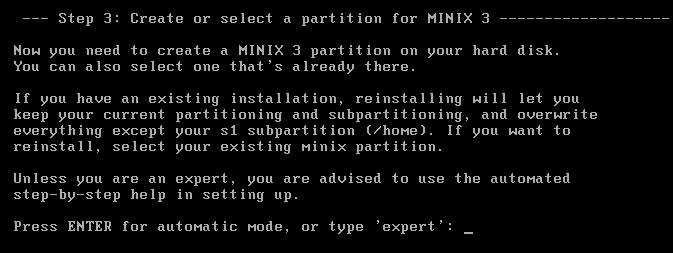
\includegraphics[width=0.7\textwidth]{vm/min20.png}
  \caption{Creación de partición}
\end{figure}

Seleccionar el único disco disponible para la instalación.
\begin{figure}[H]
  \centering
  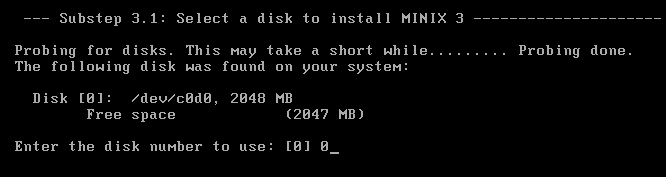
\includegraphics[width=0.7\textwidth]{vm/min21.png}
  \caption{Selección de disco}
\end{figure}

Confirmar las opciones seleccionadas ingresando la palabra \texttt{yes}.
\begin{figure}[H]
  \centering
  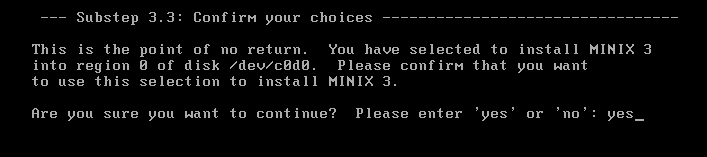
\includegraphics[width=0.7\textwidth]{vm/min22.png}
  \caption{Confirmacion de opciones}
\end{figure}

\subsubsection{Tamaño del directorio \textit{/home}}
Indicar cuál será el tamaño de \texttt{/home}.
\begin{figure}[H]
  \centering
  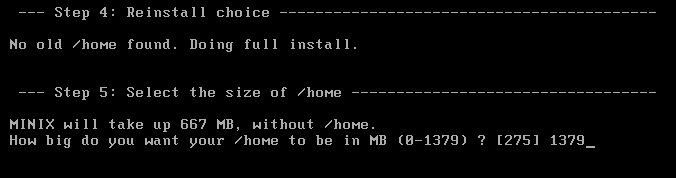
\includegraphics[width=0.7\textwidth]{vm/min24.png}
  \caption{Configuración de tamaño de \texttt{/home}}
\end{figure}

\subsubsection{Tamaño de bloque}
Seleccionar cuál será el tamaño de los bloques, en este caso se dejó el tamaño por defecto de 4KB.
\begin{figure}[H]
  \centering
  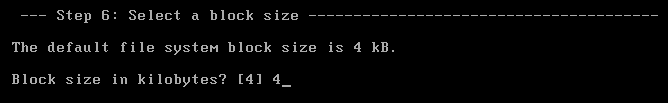
\includegraphics[width=0.7\textwidth]{vm/min26.png}
  \caption{Selección de tamaño de bloques}
\end{figure}

\subsubsection{Controlador de tarjeta de red}
Seleccionar el tipo de tarjeta de red en uso, en este caso se escogió la opción número 9.
\begin{figure}[H]
  \centering
  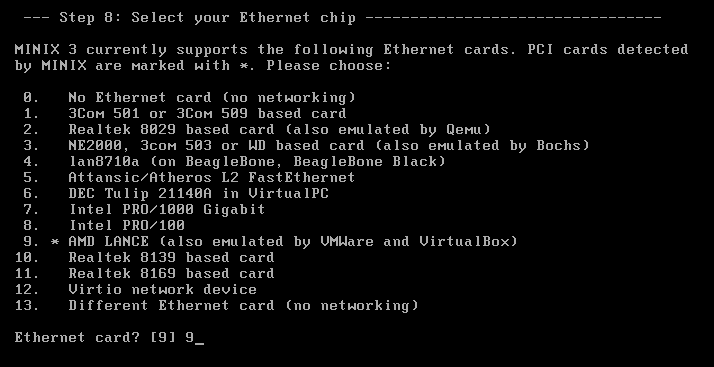
\includegraphics[width=0.7\textwidth]{vm/min27.png}
  \caption{Selección del tipo de tarjeta de red}
\end{figure}

Indicar que se utilice el protocolo \texttt{DHCP} para la configuración automática de la interfaz de red.
\begin{figure}[H]
  \centering
  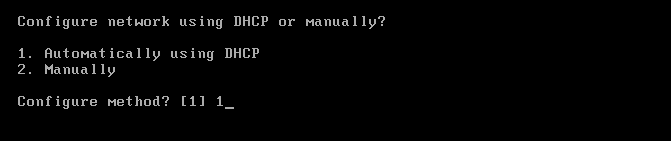
\includegraphics[width=0.7\textwidth]{vm/min30.png}
  \caption{Selección de modo de configuración de interfaz de red}
\end{figure}

\subsection{Apagado del sistema (Fin)}
Apagar máquina con el comando \texttt{poweroff} y reiniciarla siguiendo las instrucciones del virtualizador correspondiente:
\begin{itemize}
\item Ver \ref{vm:post} para iniciar la máquina con \textit{Minix} instalado en \textbf{VMWare}.
\item Ver \ref{vb:post} para iniciar la máquina con \textit{Minix} instalado en \textbf{VirtualBox}.
\end{itemize}
\begin{figure}[H]
  \centering
  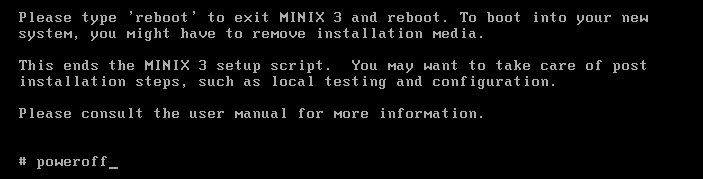
\includegraphics[width=0.7\textwidth]{vm/min31.png}
  \caption{Apagado de la máquina}
\end{figure}

\end{document}
